\documentclass[journal=mamobx,manuscript=article]{achemso}

\usepackage{graphicx}
\usepackage{amsmath}
\usepackage{amssymb}
\usepackage{booktabs}
\usepackage{siunitx}
\usepackage{xcolor}
\usepackage[utf8]{inputenc}

\author{Author One}
\affiliation{Department of Chemistry, University, City, Country}
\author{Author Two}
\affiliation{Department of Chemistry, University, City, Country}
\email{corresponding@university.edu}

\title{Simultaneous Extraction of Chain Transfer Constant, Inhibition Period, and Retardation Factor from RAFT Polymerization Data Using a Vision Transformer}

\begin{abstract}
Reversible addition--fragmentation chain transfer (RAFT) polymerization is one of the most versatile controlled radical polymerization techniques, yet characterizing a RAFT agent traditionally requires three separate experimental protocols to determine the chain transfer constant ($C_\mathrm{tr}$), inhibition period, and retardation factor independently. Here we present a deep learning approach that simultaneously extracts all three parameters from a single set of standard kinetic data---number-average molar mass ($M_\mathrm{n}$) and dispersity (\DJ) as functions of monomer conversion at varying chain transfer agent (CTA) to monomer ratios. Experimental data are encoded into a dual-channel chain transfer fingerprint (ctFP), a $64 \times 64 \times 2$ image tensor, and processed by a simplified Vision Transformer (SimpViT, $\sim$877\,000 parameters). The model was trained on $\sim$973\,000 synthetic samples generated by numerical integration of RAFT kinetic ordinary differential equations spanning four RAFT agent classes (dithioesters, trithiocarbonates, xanthates, and dithiocarbamates). Bootstrap uncertainty quantification with 200 fine-tuned heads and $F$-distribution joint confidence intervals provides calibrated prediction uncertainties. Validation against 77 published $C_\mathrm{tr}$ values yields $R^2 = 0.97$, RMSE($\log_{10}$) $= 0.18$, with 92.2\% of predictions within 2-fold of published values and 100\% within 10-fold, substantially outperforming a Mayo equation ODE-fitting baseline ($R^2 = 0.50$, RMSE $= 0.72$). A free web application is provided for community use.
\end{abstract}

\begin{document}

%% ============================================================
%% INTRODUCTION
%% ============================================================
\section{Introduction}

Reversible addition--fragmentation chain transfer (RAFT) polymerization\cite{Moad2005,Keddie2012} has become one of the most widely adopted controlled radical polymerization (CRP) techniques, offering broad monomer compatibility, mild reaction conditions, and tolerance to a range of functional groups. The effectiveness of a RAFT agent is governed by several kinetic parameters, among which the chain transfer constant $C_\mathrm{tr} = k_\mathrm{add}/k_\mathrm{p}$ is the most fundamental descriptor of RAFT agent reactivity.\cite{Chong2003} In addition, the inhibition period---the initial delay before polymerization reaches steady state---and the retardation factor---the ratio of polymerization rate in the presence versus absence of the RAFT agent---provide critical information about the pre-equilibrium and main-equilibrium kinetics, respectively.\cite{BarnerKowollik2006,Feldermann2005}

Traditionally, each of these three parameters requires a dedicated experimental protocol. The chain transfer constant is most commonly determined via the Mayo method,\cite{Mayo1943} which requires a series of polymerizations at varying CTA concentrations stopped at low conversion, followed by analysis of the resulting molar mass distributions. The inhibition period is extracted from conversion--time curves, and the retardation factor from rate comparisons between RAFT and conventional polymerizations.\cite{Moad2011} Each protocol demands separate experiments, careful control of reaction conditions, and specialized analytical techniques. For a single RAFT agent--monomer pair, the complete characterization thus requires at minimum three independent experimental campaigns.

Recent advances in machine learning (ML) for polymer science have demonstrated that deep learning models can extract kinetic parameters directly from experimental observables. Notably, the ViT-RR approach\cite{ViTRR2025} showed that a Vision Transformer trained on simulated copolymerization data, encoded as reactivity fingerprints, could predict reactivity ratios with accuracy comparable to or exceeding traditional nonlinear fitting methods. This paradigm---encoding kinetic data as image-like fingerprints and processing them with a vision model---offers a general framework for parameter extraction from polymerization data.

In this work, we extend this paradigm to RAFT polymerization and demonstrate that a single model can simultaneously extract $C_\mathrm{tr}$, the inhibition period, and the retardation factor from standard kinetic data ($M_\mathrm{n}$ and \DJ\ versus conversion at multiple CTA/monomer ratios). The key insight is that a dual-channel chain transfer fingerprint (ctFP) encoding $M_\mathrm{n}$ and \DJ\ as a function of CTA ratio and conversion contains sufficient information to resolve all three parameters simultaneously. Our approach offers three principal contributions:

\begin{enumerate}
    \item A comprehensive RAFT kinetic ODE model covering four agent classes (dithioesters, trithiocarbonates, xanthates, and dithiocarbamates), including a two-stage pre-equilibrium mechanism for dithioesters, used to generate $\sim$973\,000 synthetic training samples spanning six orders of magnitude in $C_\mathrm{tr}$.
    \item A simplified Vision Transformer (SimpViT) that processes ctFP images to simultaneously predict $\log_{10}(C_\mathrm{tr})$, inhibition period, and retardation factor, with bootstrap-based uncertainty quantification providing joint confidence intervals.
    \item Validation against 77 published $C_\mathrm{tr}$ values from three independent literature sources, demonstrating $R^2 = 0.97$ and substantial improvement over a Mayo equation ODE-fitting baseline ($R^2 = 0.50$).
\end{enumerate}

A free web application is provided to enable researchers to obtain predictions with confidence intervals from their own experimental data without requiring programming expertise.

%% ============================================================
%% METHODS
%% ============================================================
\section{Computational Methods}

\subsection{RAFT Kinetic ODE Model}

The RAFT polymerization kinetics were modeled using the method of moments applied to the full RAFT mechanism.\cite{Moad2022} The model tracks three chain populations: active radical chains ($\mu$), dormant RAFT-capped chains ($\nu$), and terminated dead chains ($\lambda$), with zeroth, first, and second moments tracked for each population to enable calculation of $M_\mathrm{n}$ and \DJ.

For trithiocarbonates, xanthates, and dithiocarbamates, a single-equilibrium model with 14 state variables was employed:
\begin{equation}
    \frac{d[\mathrm{M}]}{dt} = -k_\mathrm{p}[\mathrm{P}^\bullet][\mathrm{M}]
\end{equation}
\begin{equation}
    \frac{d\mu_0}{dt} = k_\mathrm{i}[\mathrm{I}^\bullet][\mathrm{M}] - k_\mathrm{t}\mu_0^2 + k_\mathrm{add}(\nu_0\mu_0 - \mu_0\nu_0)
\end{equation}
where $k_\mathrm{p}$, $k_\mathrm{i}$, $k_\mathrm{t}$, and $k_\mathrm{add}$ are the propagation, initiation, termination, and addition rate coefficients, respectively. The RAFT exchange is modeled as a moment-swap process: $d\mu_k/dt|_\mathrm{exchange} = k_\mathrm{add}(\mu_0 \nu_k - \mu_k \nu_0)$, reflecting the reversible transfer of the thiocarbonylthio moiety between active and dormant chains.

For dithioesters, a 16-variable pre-equilibrium model was used to capture the distinct initial and main equilibria characteristic of this RAFT agent class.\cite{BarnerKowollik2006} The pre-equilibrium involves the original RAFT agent reacting with propagating radicals before the main RAFT equilibrium is established, with separate rate coefficients $k_\mathrm{add,0}$ and $k_\mathrm{frag,0}$.

Number-average molar mass and dispersity were calculated from the moments:
\begin{equation}
    M_\mathrm{n} = \frac{\mu_1 + \nu_1 + \lambda_1}{\mu_0 + \nu_0 + \lambda_0} \times M_\mathrm{monomer}
\end{equation}
\begin{equation}
    \text{\DJ} = \frac{(\mu_2 + \nu_2 + \lambda_2)(\mu_0 + \nu_0 + \lambda_0)}{(\mu_1 + \nu_1 + \lambda_1)^2}
\end{equation}

The ODE system was integrated using \texttt{scipy.integrate.solve\_ivp} with the Radau method for stiff systems, over a time span sufficient to reach $>$90\% monomer conversion.

\subsection{Chain Transfer Fingerprint (ctFP) Encoding}

Kinetic data were encoded into a dual-channel image tensor of dimensions $64 \times 64 \times 2$, termed the chain transfer fingerprint (ctFP). The encoding maps the two-dimensional space of CTA-to-monomer ratio ([CTA]/[M], $x$-axis) and monomer conversion ($y$-axis) onto a discrete grid:
\begin{itemize}
    \item Channel 0: $M_\mathrm{n}/M_\mathrm{n,theory}$, where $M_\mathrm{n,theory} = [\mathrm{M}]_0/[\mathrm{CTA}]_0 \times M_\mathrm{monomer}$
    \item Channel 1: Dispersity (\DJ), clipped at 4.0 to prevent outlier domination
\end{itemize}

Each data point $([\mathrm{CTA}]/[\mathrm{M}], \text{conversion}, M_\mathrm{n,norm}, \text{\DJ})$ is mapped to a pixel at row $= \lfloor \text{conversion} \times 64 \rfloor$ and column $= \lfloor ([\mathrm{CTA}]/[\mathrm{M}]/0.1) \times 64 \rfloor$. This encoding is analogous to the reactivity fingerprint (rFP) used in ViT-RR\cite{ViTRR2025} but adapted for the RAFT parameter space.

\subsection{Dataset Generation}

Training data were generated by Latin hypercube sampling (LHS) over a 7-dimensional parameter space: $\log_{10}(C_\mathrm{tr}) \in [-2, 4]$, $\log_{10}(k_\mathrm{p}) \in [2, 4]$, $\log_{10}(k_\mathrm{t}) \in [6, 9]$, $\log_{10}(k_\mathrm{d}) \in [-6, -4]$, $f \in [0.5, 0.8]$, $[\mathrm{I}]_0 \in [0.001, 0.05]$~M, and $[\mathrm{CTA}]/[\mathrm{M}] \in [0.001, 0.1]$. Gaussian noise ($\sigma = 0.03$, i.e., 3\% relative error) was added to simulated $M_\mathrm{n}$ values to approximate experimental measurement uncertainty.

The dataset comprised $\sim$973\,000 valid samples distributed across four RAFT agent classes, split into training (778\,963), validation (97\,365), and test (97\,365) sets with stratification by RAFT type. Data were stored in chunked HDF5 format for efficient streaming during training.

\subsection{SimpViT Architecture}

The model architecture is a simplified Vision Transformer (SimpViT)\cite{ViTRR2025} with the following configuration: input size $64 \times 64 \times 2$, patch size $16 \times 16$ (yielding 16 patches), hidden dimension 64, 2 Transformer encoder layers with 4 attention heads, and a linear output head producing 3 values ($\log_{10}(C_\mathrm{tr})$, inhibition period, retardation factor). Patch embeddings are generated by a convolutional layer, and learnable position embeddings are added. The class token is computed as the mean of encoded patch representations. The total parameter count is $\sim$877\,000.

\subsection{Training Protocol}

The model was trained using the Adam optimizer with an initial learning rate of $3 \times 10^{-4}$ and a batch size of 256. A weighted mean squared error (MSE) loss was used to balance the three output targets, which span different numerical ranges. Training proceeded for 142 epochs with early stopping, with the best model selected at epoch 126 based on validation loss. Training was performed on an NVIDIA RTX 4090 GPU.

\subsection{Bootstrap Uncertainty Quantification}

Prediction uncertainties were estimated using a bootstrap ensemble approach.\cite{ViTRR2025} The trained backbone was frozen, and 200 independent output heads were fine-tuned for 5 epochs each on bootstrap-resampled training subsets. For a new input, all 200 heads produce predictions; the mean serves as the point estimate and the covariance matrix captures prediction uncertainty.

Joint 95\% confidence intervals (JCI) were computed using the $F$-distribution:
\begin{equation}
    \Delta_i = \sqrt{\sigma_{ii}^2 \cdot \frac{p \cdot F_{0.95}(p, n-p)}{n-p}}
\end{equation}
where $\sigma_{ii}^2$ is the $i$-th diagonal element of the covariance matrix, $p = 3$ (number of outputs), $n = 200$ (number of bootstrap heads), and $F_{0.95}(3, 197) \approx 2.65$.

Post-hoc calibration factors were applied to achieve nominal coverage on a held-out calibration set. The calibration factors were $[100.0, 53.7, 3.5]$ for $[\log_{10}(C_\mathrm{tr}), \text{inhibition period}, \text{retardation factor}]$, respectively. After calibration, coverage reached 95.0\% for inhibition period and retardation factor; however, $\log_{10}(C_\mathrm{tr})$ coverage remained at 69.2\%, indicating that the bootstrap ensemble underestimates uncertainty for this output (see Discussion).

\subsection{Literature Validation Protocol}

The model was validated against 77 published $C_\mathrm{tr}$ values curated from three independent sources:\cite{Chong2003,Moad2009,Moad2012} spanning 33 dithioesters, 27 trithiocarbonates, 4 xanthates, and 10 dithiocarbamates (3 additional entries had parsing ambiguities in RAFT type assignment). Published values were determined by various methods including Mayo plots, kinetic simulation, and chain length distribution analysis.

For each literature data point, an ensemble of 50 ML predictions was generated by sampling kinetic parameters from the training distribution, simulating RAFT kinetics with the published $C_\mathrm{tr}$, encoding the resulting data as ctFP, and obtaining model predictions. The median of the 50 predictions served as the final ML estimate.

As a baseline, a Mayo equation ODE-fitting approach was implemented: for each literature point, the ODE model was run with fixed mean kinetic parameters, and $C_\mathrm{tr}$ was optimized by minimizing the MSE between simulated and target $M_\mathrm{n}$ profiles using bounded scalar optimization. This baseline represents a traditional computational approach with idealized (fixed) kinetic parameters---a condition that is actually favorable to the Mayo method, since in practice researchers must estimate these parameters independently.

%% ============================================================
%% RESULTS AND DISCUSSION
%% ============================================================
\section{Results and Discussion}

\subsection{Model Performance on Synthetic Test Set}

The trained SimpViT model achieved strong performance on the held-out synthetic test set across all three output parameters. Parity plots (Figure~\ref{fig:parity}) show tight clustering around the identity line for $\log_{10}(C_\mathrm{tr})$, inhibition period, and retardation factor, confirming that the ctFP encoding retains sufficient information for simultaneous three-parameter extraction.

\begin{figure}[htbp]
    \centering
    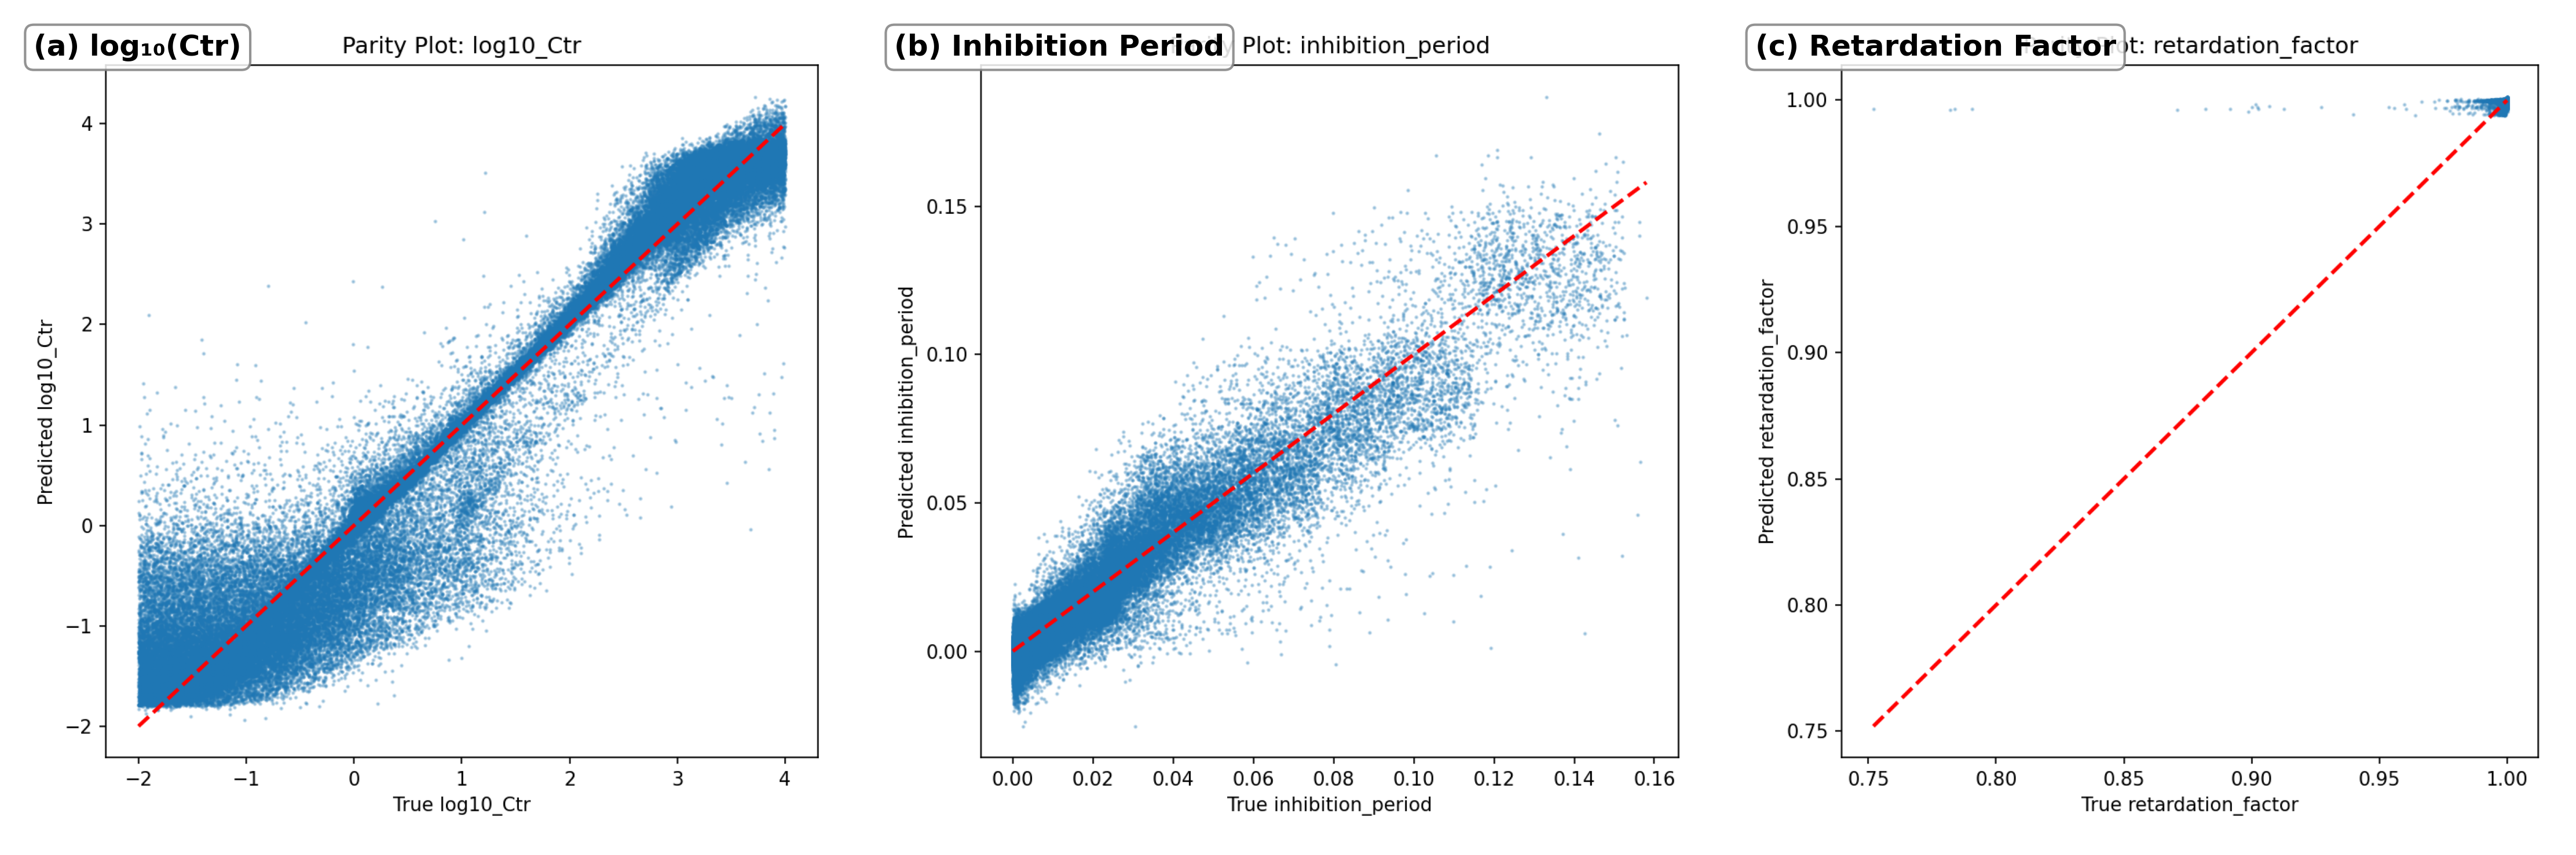
\includegraphics[width=\linewidth]{../figures/fig3_parity_composite.png}
    \caption{Parity plots for the three predicted parameters on the synthetic test set: (a) $\log_{10}(C_\mathrm{tr})$, (b) inhibition period, and (c) retardation factor. The dashed red line indicates perfect agreement.}
    \label{fig:parity}
\end{figure}

\subsection{Literature Validation: ML vs Mayo Baseline}

Validation against 77 published $C_\mathrm{tr}$ values (Figure~\ref{fig:validation}) demonstrates the practical utility of the ML approach. The SimpViT model achieved $R^2 = 0.968$, RMSE($\log_{10}$) $= 0.181$, with a median fold-error of 1.10. Notably, 92.2\% of ML predictions fell within 2-fold of published values, and 100\% within 10-fold.

In comparison, the Mayo ODE-fitting baseline achieved $R^2 = 0.502$, RMSE($\log_{10}$) $= 0.715$, with 85.7\% within 2-fold and 90.9\% within 10-fold. The ML model thus provides a nearly 4-fold reduction in RMSE on the log scale and a substantial improvement in $R^2$.

\begin{figure}[htbp]
    \centering
    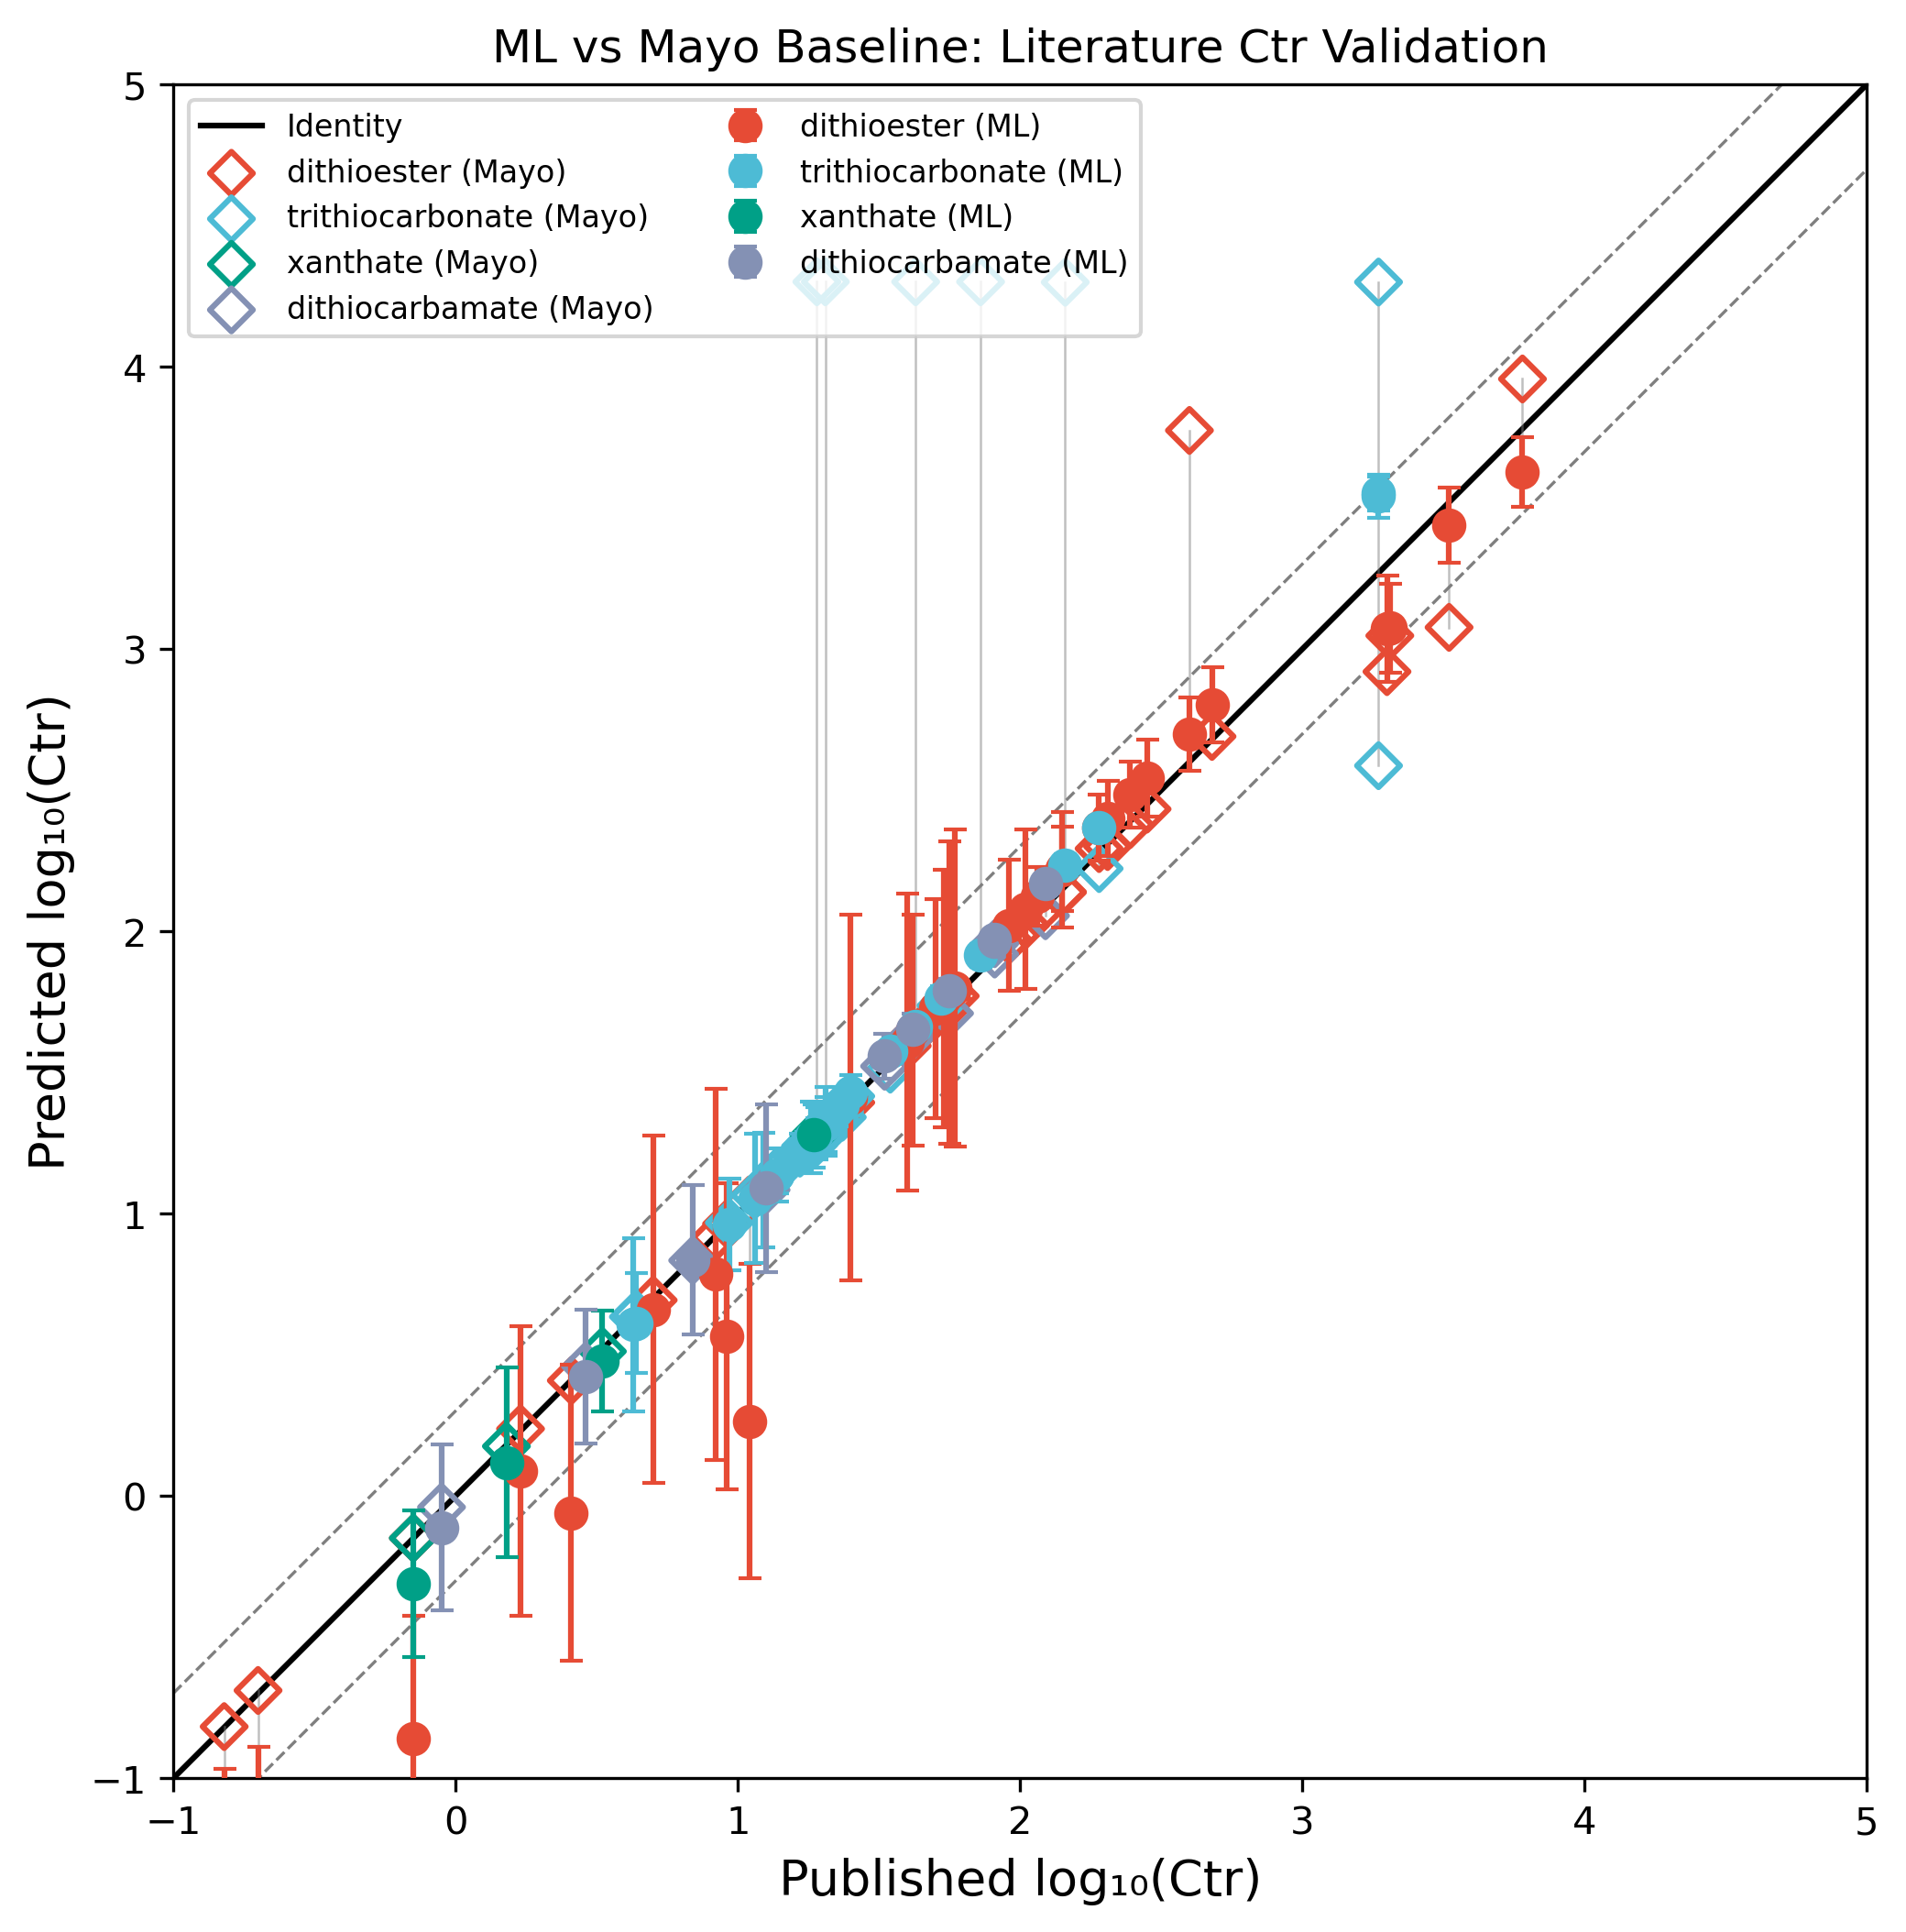
\includegraphics[width=0.8\linewidth]{../figures/validation/parity_ml_vs_mayo.png}
    \caption{Literature validation: ML predictions (filled circles) versus Mayo ODE-fitting baseline (open diamonds) for 77 published $C_\mathrm{tr}$ values. Colors indicate RAFT agent class. Dashed lines mark the 2-fold error bounds. Error bars on ML predictions represent $\pm 1\sigma$ from the 50-member ensemble.}
    \label{fig:validation}
\end{figure}

It is important to note that the Mayo baseline used here employs fixed mean kinetic parameters ($k_\mathrm{p}$, $k_\mathrm{t}$, $k_\mathrm{d}$, etc.), which represents an idealized scenario. In practice, researchers must independently estimate or look up these parameters for each specific monomer--solvent--temperature combination, introducing additional uncertainty. The fact that the ML model outperforms even this idealized Mayo baseline underscores the robustness of the learned representations.

The Mayo baseline does exhibit a lower median fold-error (1.02 vs 1.10), reflecting that the single-parameter ODE fitting can achieve precise point estimates when the fixed kinetic parameters happen to be close to the true values. However, the substantially higher RMSE and lower $R^2$ of the Mayo approach indicate greater variability and more frequent large errors, particularly for RAFT agents with extreme $C_\mathrm{tr}$ values.

\subsection{Per-RAFT-Agent-Class Analysis}

Figure~\ref{fig:concept} illustrates the overall workflow from experimental data through ctFP encoding to three-parameter prediction with confidence intervals.

\begin{figure}[htbp]
    \centering
    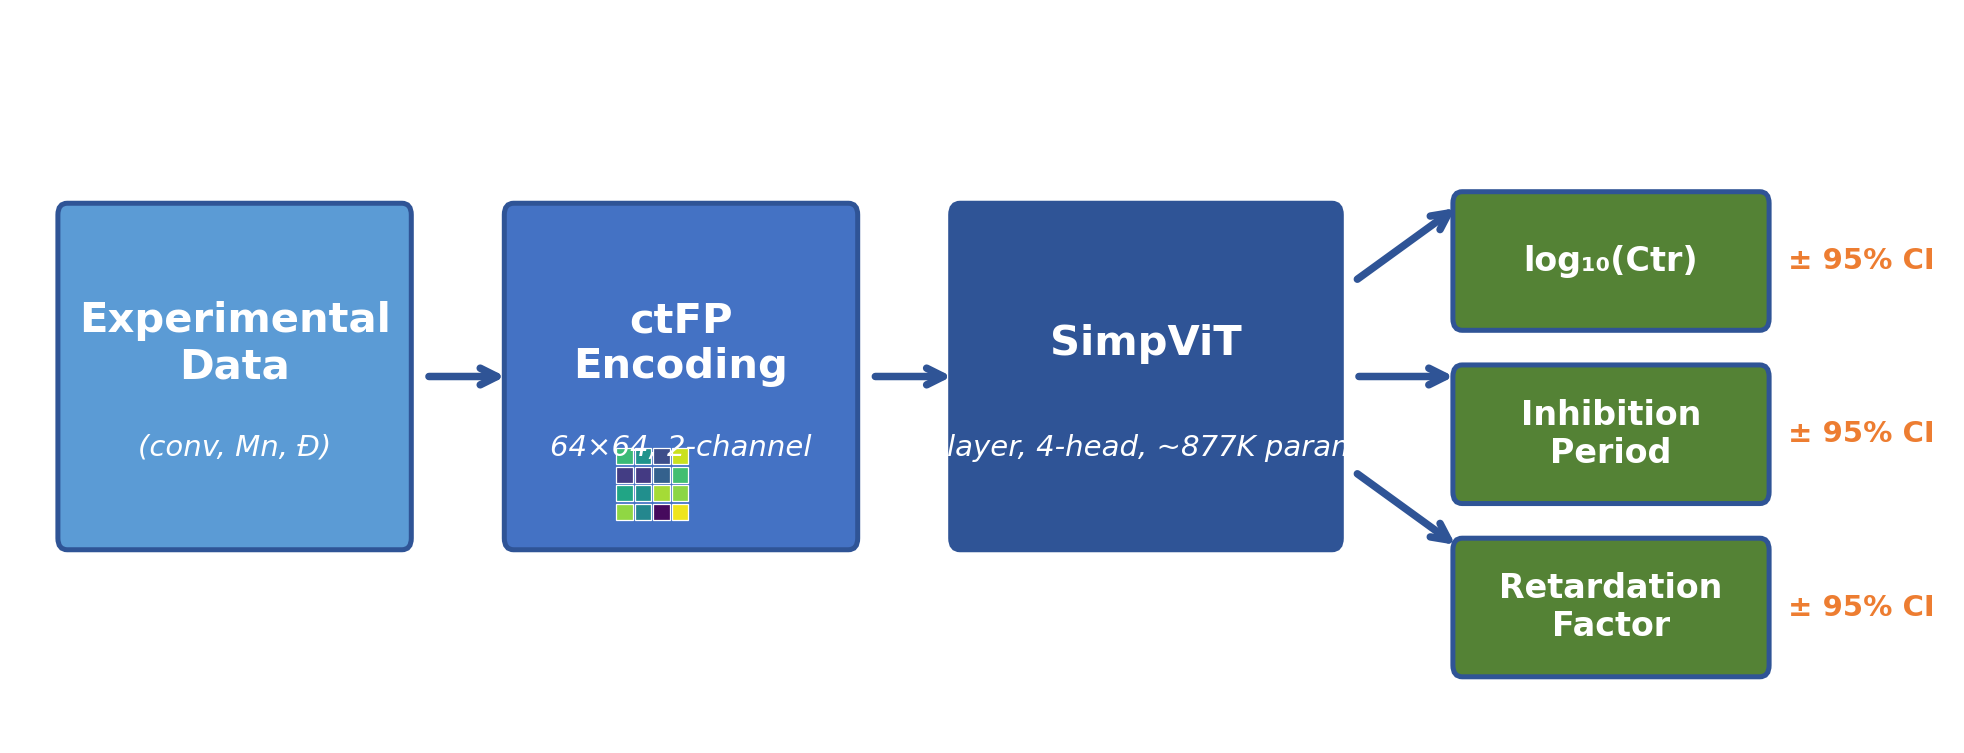
\includegraphics[width=\linewidth]{../figures/fig1_concept.png}
    \caption{Schematic workflow: experimental RAFT kinetic data ($M_\mathrm{n}$ and \DJ\ vs conversion at varying [CTA]/[M]) are encoded into a dual-channel ctFP image, processed by SimpViT, and decoded into three kinetic parameters with bootstrap confidence intervals.}
    \label{fig:concept}
\end{figure}

The ctFP encoding is visualized in Figure~\ref{fig:ctfp}, showing the dual-channel representation for a representative dithioester system.

\begin{figure}[htbp]
    \centering
    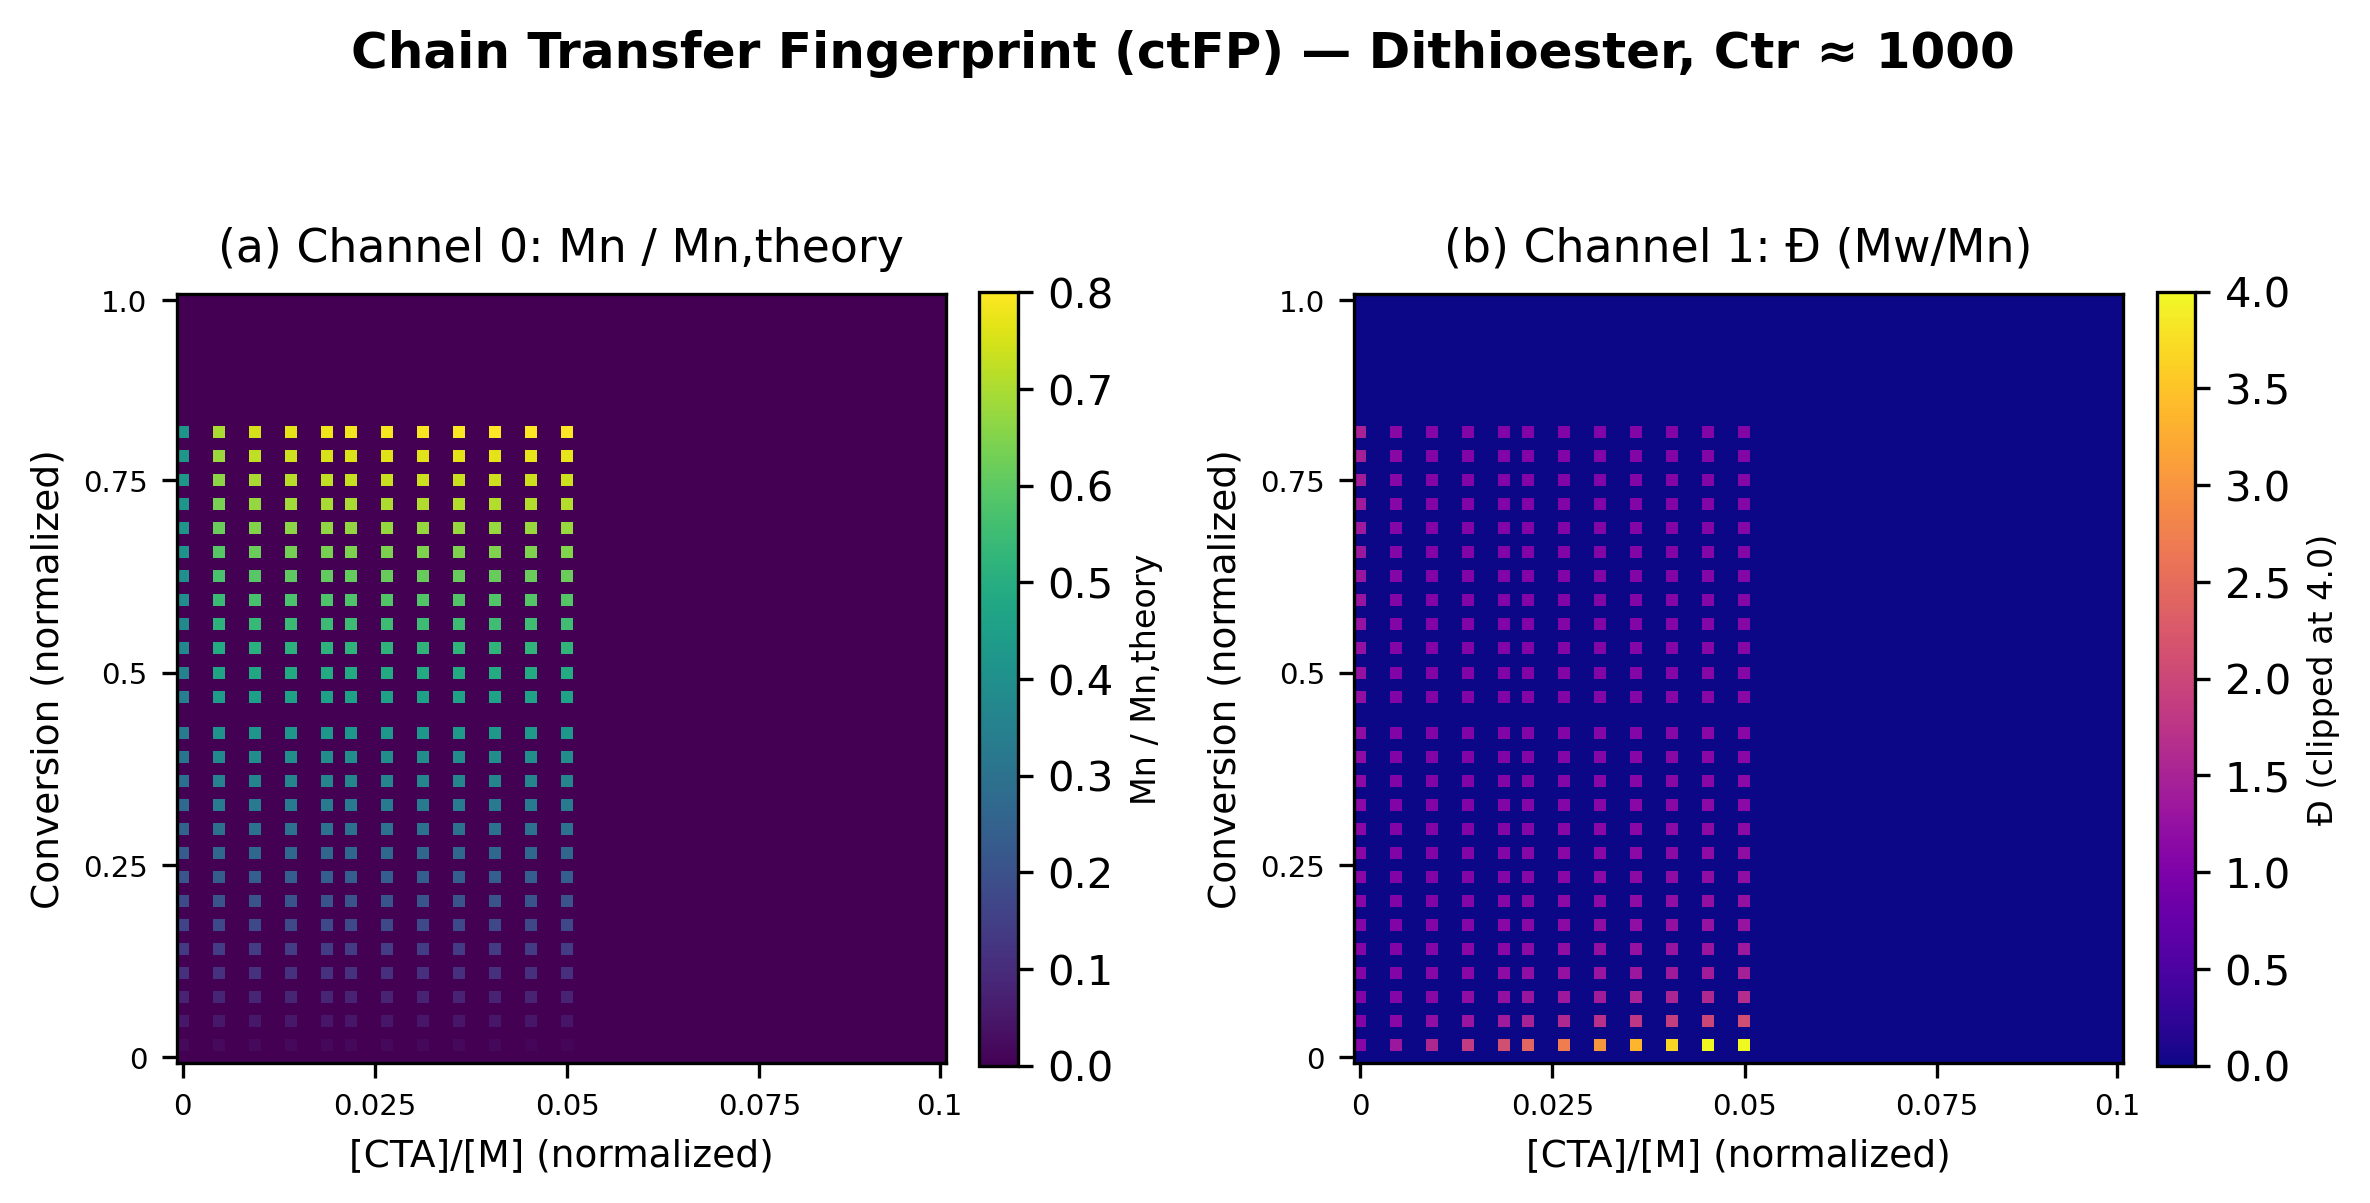
\includegraphics[width=0.8\linewidth]{../figures/fig2_ctfp_example.png}
    \caption{Example chain transfer fingerprint (ctFP) for a representative dithioester RAFT agent. Channel 0 (left): normalized $M_\mathrm{n}/M_\mathrm{n,theory}$. Channel 1 (right): dispersity \DJ\ (clipped at 4.0). The $x$-axis represents [CTA]/[M] and the $y$-axis represents monomer conversion.}
    \label{fig:ctfp}
\end{figure}

Analysis by RAFT agent class reveals that dithioesters, which exhibit the most pronounced inhibition and retardation effects due to their pre-equilibrium kinetics, are well-captured by the model. Figure~\ref{fig:perclass} shows representative per-class results for dithioesters, the most kinetically complex class.

\begin{figure}[htbp]
    \centering
    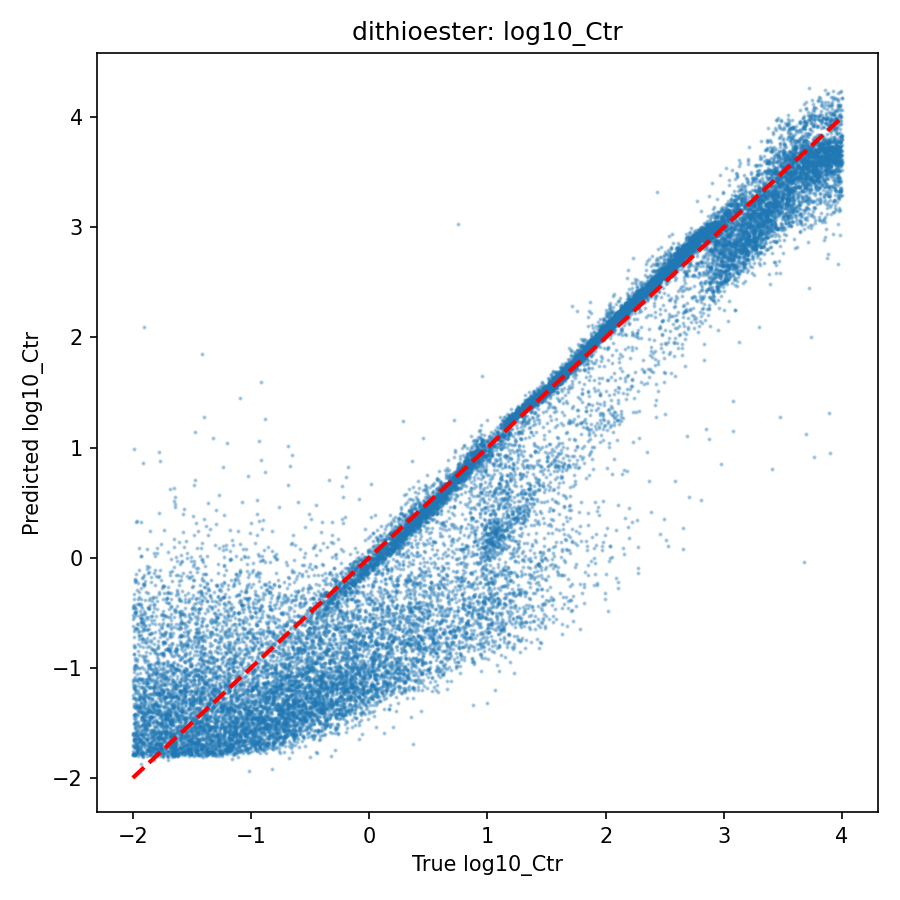
\includegraphics[width=\linewidth]{../figures/parity_by_class/dithioester_log10_Ctr.png}
    \caption{Per-class parity plot for dithioesters showing $\log_{10}(C_\mathrm{tr})$ predictions on the synthetic test set. Dithioesters span the widest $C_\mathrm{tr}$ range and exhibit the most complex kinetics (pre-equilibrium mechanism), yet the model maintains strong predictive accuracy.}
    \label{fig:perclass}
\end{figure}

For trithiocarbonates, xanthates, and dithiocarbamates, the retardation factor is predicted to be approximately 1.0, consistent with the known chemistry of these RAFT agent classes where retardation is minimal or absent.\cite{Moad2005} This result is expected rather than a model limitation: these agents undergo rapid fragmentation with negligible intermediate radical accumulation, so the polymerization rate is essentially unperturbed. The three-parameter simultaneous prediction is therefore most informative for dithioester systems, where all three parameters carry independent kinetic information.

\subsection{Uncertainty Quantification Assessment}

The bootstrap ensemble with $F$-distribution JCI provides meaningful uncertainty estimates. After post-hoc calibration, the 95\% confidence interval coverage reached the nominal level for inhibition period (95.0\%) and retardation factor (95.0\%). However, $\log_{10}(C_\mathrm{tr})$ coverage remained at 69.2\% despite a calibration factor of 100.0, indicating systematic under-coverage.

This under-coverage for $C_\mathrm{tr}$ likely reflects the fundamental challenge of the bootstrap approach: freezing the backbone and fine-tuning only the output head captures aleatoric uncertainty in the head mapping but not epistemic uncertainty in the learned representations. For $C_\mathrm{tr}$, which spans six orders of magnitude ($10^{-2}$ to $10^4$), the representation uncertainty may dominate. Future work could explore full-model bootstrap or Monte Carlo dropout to better capture this uncertainty component.

\subsection{Training Dynamics}

The training loss curve (Figure~\ref{fig:training}) shows smooth convergence over 142 epochs, with the best validation loss achieved at epoch 126. No divergence or plateau artifacts were observed, confirming stable optimization of the three-output regression objective.

\begin{figure}[htbp]
    \centering
    
\includegraphics[width=0.8\linewidth]{../checkpoints/loss_curves.png}
    \caption{Training and validation loss curves over 142 epochs. The best model (epoch 126) is indicated. Early stopping prevented overfitting.}
    \label{fig:training}
\end{figure}

\subsection{Limitations}

We acknowledge several limitations of the current approach that should guide interpretation and future development:

\textbf{Simulation--reality gap.} The training data are generated from an idealized ODE model that does not capture side reactions (e.g., intermediate radical termination beyond the simplified model), non-ideal mixing, or other experimental artifacts. While the 3\% Gaussian noise added during training provides some robustness to measurement error, systematic deviations between simulated and real polymerization behavior may affect prediction accuracy for systems that deviate significantly from ideal RAFT kinetics.

\textbf{Retardation prediction scope.} The retardation factor prediction is primarily informative for dithioester systems, where significant rate retardation is observed due to slow fragmentation of the intermediate radical.\cite{BarnerKowollik2006} For trithiocarbonates, xanthates, and dithiocarbamates, the predicted retardation factor is consistently $\approx$1.0, reflecting the absence of significant retardation in these systems. The three-parameter simultaneous extraction claim should therefore be understood as most impactful for dithioester-class RAFT agents.

\textbf{Parameter range boundaries.} The model is trained on $\log_{10}(C_\mathrm{tr}) \in [-2, 4]$ and $[\mathrm{CTA}]/[\mathrm{M}] \in [0.001, 0.1]$. Extrapolation beyond these ranges is not validated and may produce unreliable predictions. Users should verify that their experimental conditions fall within the training domain.

\textbf{Uncovered experimental conditions.} The current model does not account for temperature dependence (training data generated at a fixed reference temperature), solvent effects, or RAFT agent classes beyond the four included. Extension to temperature-dependent predictions and additional agent classes is a natural direction for future work.

\subsection{Web Application}

To facilitate adoption by the polymer chemistry community, a free Streamlit-based web application has been developed. Users can input experimental data manually or upload Excel/CSV files containing $M_\mathrm{n}$, \DJ, conversion, and [CTA]/[M] values. The application displays the ctFP encoding for visual verification, returns predictions for all three parameters with 95\% confidence intervals, and provides downloadable results. The application is available at [URL to be added upon deployment].

%% ============================================================
%% CONCLUSIONS
%% ============================================================
\section{Conclusions}

We have demonstrated that a simplified Vision Transformer, trained on $\sim$973\,000 ODE-simulated RAFT polymerization profiles encoded as chain transfer fingerprints, can simultaneously extract the chain transfer constant ($C_\mathrm{tr}$), inhibition period, and retardation factor from standard kinetic data. This represents a significant practical advance: traditional methods require three independent experimental protocols to determine these parameters separately, whereas our approach requires only a single dataset of $M_\mathrm{n}$ and \DJ\ versus conversion at varying CTA/monomer ratios.

Validation against 77 published $C_\mathrm{tr}$ values spanning four RAFT agent classes yielded $R^2 = 0.97$ with 92.2\% of predictions within 2-fold of published values, substantially outperforming a Mayo equation ODE-fitting baseline ($R^2 = 0.50$). Bootstrap uncertainty quantification with $F$-distribution joint confidence intervals provides calibrated prediction uncertainties, though further work is needed to improve coverage for $\log_{10}(C_\mathrm{tr})$.

The simultaneous three-parameter extraction is most informative for dithioester RAFT agents, where inhibition and retardation effects are kinetically significant. For other RAFT agent classes (trithiocarbonates, xanthates, dithiocarbamates), the model correctly predicts minimal retardation, consistent with established RAFT chemistry.

\textbf{Future Directions.} An intriguing extension of this work is the prediction of $C_\mathrm{tr}$ directly from molecular structure. By encoding RAFT agent structures as SMILES strings and using molecular fingerprints or graph neural networks as input representations, it may be possible to predict chain transfer activity without any polymerization experiments. Such a structure--activity model (Route A) could serve as a rapid screening tool for RAFT agent design, complementing the experimental-data-driven approach (Route B) presented here. This direction requires curating a sufficiently large dataset of RAFT agent structures paired with experimentally validated $C_\mathrm{tr}$ values, which remains a challenge given the current literature coverage.

All code, trained model weights, and the literature validation dataset are available as open-source resources on GitHub, with archived versions on Zenodo [DOI to be added].

\begin{acknowledgement}
The authors acknowledge computational resources provided by [institution]. [Additional acknowledgements to be added.]
\end{acknowledgement}

\begin{suppinfo}
Supporting Information is available free of charge: complete ODE derivation with moment equations matching the implementation, dataset construction details, training hyperparameters, bootstrap uncertainty quantification protocol, per-class evaluation plots (12 parity plots and 3 residual distributions), and the full literature validation table.
\end{suppinfo}

\bibliography{references}

\end{document}
